\documentclass{article}
\usepackage[utf8]{inputenc}
\usepackage[portuges]{babel}
\usepackage{graphicx}
% citacoes em abnt 2 6063:2002
\usepackage[num]{abntex2cite}

% configurações de fonte
\usepackage{times}
\documentclass[12pt]{report}

%margin settings
\usepackage{geometry}
 \geometry{
 a4paper,
 left=30mm,
 right=20mm,
 top=30mm,
 bottom=20mm,
 }

\usepackage{index}
\renewcommand{\baselinestretch}{1.50}\normalsize
% custom variables
\newcommand{\publicationDate}{Dezembro 2014}
\newcommand{\tccTitle}{Problemas no desenvolvimento de jogos 2D em HTML5}
% end - custom variables
\renewcommand{\paragraph}{%
  \@startsection{paragraph}{4}%
  {\z@}{3.25ex \@plus 1ex \@minus .2ex}{-1em}%
  {\normalfont\normalsize\bfseries}%
}
\parskip 7.2pt
\parindent 8pt

\newfloat{figure}{thp}{lop}
\floatname{figure}{Figure}

\begin{document}


\begin{titlepage}
    \begin{center}
        {\large INSTITUTO FEDERAL DE EDUCAÇÃO, CIÊNCIA E TECNOLOGIA DO RIO GRANDE DO SUL } \\
        {\large CÂMPUS BENTO GONÇALVES-RS} \\[4.9cm]
        {\large Jean Carlo Machado} \\[4.9cm]
        {\Huge \tccTitle{}} \\[4.9cm]
        \vfill
        {\large Bento Gonçalves, \publicationDate{}}
    \end{center}
\end{titlepage}

% Folha de rosto sem o uso de \folhaderosto
\begin{titlepage}
    \begin{center}
        {\large Jean Carlo Machado} \\[2.3cm]
         {\Huge \tccTitle} \\[2.3cm]
        {\large Trabalho de conclusão de curso} \\[2.3cm]
        \hspace{.45\textwidth} % posicionando a minipage
        \begin{minipage}{.5\textwidth}
            \begin{espacosimples}
                Projeto de Pesquisa apresentado junto ao Curso de Tecnologia em Análise e Desenvolvimento de Sistemas do Instituto Federal de Educação, Ciência e Tecnologia do Rio Grande do Sul, como requisito parcial ao desenvolvimento do Trabalho de Conclusão de Curso.
                \\\\Orientador: Me. Rafael Jaques
            \end{espacosimples}
        \end{minipage}
        \vfill
        {\large Bento Gonçalves, \publicationDate{}}
    \end{center}
\end{titlepage}

\vfill
\setlength{\ABNTsignthickness}
\assinatura{}
\assinatura{}
\assinatura{}
\end{folhadeaprovacao}
\newpage

%resumo 250 palavras

\section*{RESUMO}

 
Com a introdução dos novos recursos de multimídia oferecidos pelo HTML5 a viabilidade de construção de jogos iterativos, com as tecnologias da WEB, voltou a ser assunto relevante. Esse trabalho busca avaliar as limitações e possíveis dificuldades à se enfrentar na construção de um jogo 2D utilizando HTML5 e demais tecnologias relacionadas.

Como caráter de avaliação fez-se uma pesquisa de ferramentas e utilitários disponíveis e construiu-se um jogo 2D utilizando as consideradas mais adequadas. Com base nesta experiência constatamos que...


\textbf{Palavras-chave}: HTML5, JOGOS 2D, PROBLEMAS

\newpage

\listoffigures
\listoftables
\newpage

\tableofcontents
\newpage

\section{CONTEXTUALIZAÇÃO}
\subsection{HISTÓRIA E BENEFÍCIOS DOS JOGOS}

Há muito os jogos são utilizados como meio de entretenimento mas além da diversão propiciada, estes podem ser benéficos de diversas outras formas como: apuração da capacidade lógica, motora, facilidade em tomada de decisões, redução de stress, entre outros (GALLAGHER, 2013).
\\
	Na informática, os jogos estão presentes desde meados dos anos 60; no início, apenas protótipos de laboratórios, os jogos eram aplicativos extremamente simples e totalmente dependentes da plataforma onde eram desenvolvidos.
\\
	Em 1972, com a criação da Atari, os jogos eletrônicos se popularizaram. Criou-se um mercado competitivo onde grandes corporações internacionais disputavam para disponibilizar as melhores plataformas e os melhores jogos.  Essas corporações, dentre as maiores à dizer: Nintendo, Sony e Microsoft, devido ao alto nível de competitividade do mercado, desenvolveram novas tecnologias, criaram novos conceitos, a fim de prover maior entretenimento e imersão ao usuário. Exemplos de tecnologias desenvolvidas ou melhoradas para os games são: renderizadores de elementos de 3 dimensões (3D), bibliotecas de física avançada, produções musicais específicas para os jogos, bem como o acréscimo no nível de detalhamento gráfico devido às GPU's Graphics Processing Unit's (ou unidades de processamento gráfico) mais poderosas utilizadas.
\\
	A indústria dos video games foi rejuvenescida com a introdução da Nintendo ao final nos anos 80. Com melhoras significativas  nos gráficos, no realismo, e com a introdução de jogos violentos, a Nintendo conseguiu uma dominância de mercado temporária (BUCHMAN,1996).
	Atualmente, devido à disponibilidade de internet de alta velocidade, a sofisticação das técnicas dos jogos, e a grande compatibilidade dos hardwares, aumentou-se o fluxo de entrada de dinheiro, o que está gerando um grande boom na indústria dos jogos (AK, 2012).
\\
	O mercado global de jogos cresceu de 70.5 billões de dólares em 2011 e espera chegar a 117.9 bilhões em 2015, crescendo em méia 13.7% de 2011 a 2015 (AK, 2012).


\begin{figure}[!htbp]
    \begin{center}
        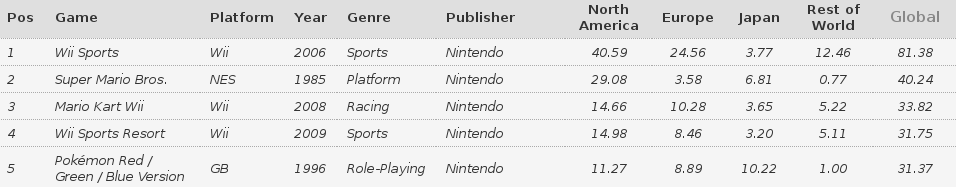
\includegraphics[width=\textwidth]{asset/img/bestSelledGames.jpg}
               \caption{Os cinco jogos mais bem vendidos de todos os tempos segundo à VGChartz, 2013) . \label{fig:Jogos mais bem vendidos}}
    \end{center}
\end{figure}

Além de obter uma estimativa de vendas dos jogos mais populares, através desta lista, é possível ter-se uma concepção de quais gêneros de jogos atraem mais os usuário. O gênero de maior influência na lista é o de esportes, seguido igualmente por plataforma, corrida e RPG.
\footnote{A VGChartz é uma bem conceituada   empresa na área de pesquisas de mercado especificamente de jogos eletrônicos.}

\subsection{Tendência smart devices}

Devido ao barateamento e miniaturalização dos componentes, tendência prevista por Moore em 1965, bem como a massificação da internet, o advento dos smart devices está em plena ascensão.

\newpage

\begin{figure}[!htbp]
    \begin{center}
        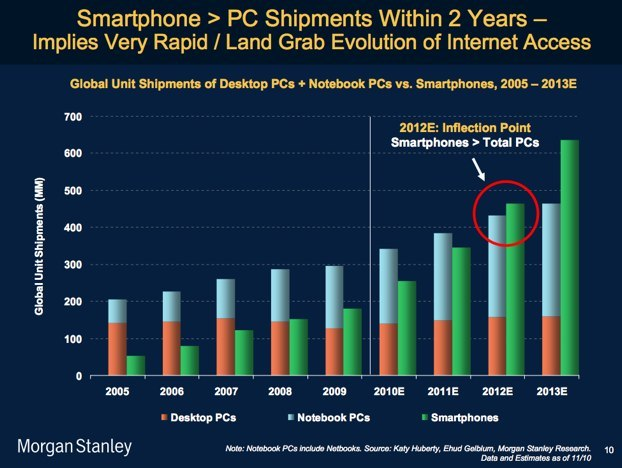
\includegraphics[width=\textwidth]{asset/img/smartvscomputer.jpg}
               \caption{Previsão de vendas de smartphones vs pc's}
    \end{center}
\end{figure}

\cite[2012, p.19]{WEINTRAUB} mostra que esta previsão se tornou realidade no último trimestre de 2010.

	Os jogos, não são a exceção em representatividade nas plataformas mobile. Segundo (HERMIDA, 2003) o total de lucros obtidos com a venda de jogos mobile ultrapassou 5,8 bilhões.
\\
	 Contudo, com a grande popularização dos smart devices - principalmente os smartphones - cada vez mais novos sistemas operacionais para estes dispositivos fazem-se disponíveis, cada qual com particularidades tais como: linguagens suportadas, recursos mínimos, tamanho de tela e aparelhos compatíveis, são exemplos de sistemas operacionais para smart-phones: Android, FirefoxOS, Ubuntu, IOS, Windows Phone. Sob esta perspectiva os desenvolvedores sentem cada vez mais o desafio que é construir aplicativos com abrangência suficiente de plataforma, de modo a alcançar todos ou a grande maioria de seus usuários (CHESTA, 2004). %REMOVE THIS CITATION
\\
	Outro desafio, não menos importante, é tornar a experiência dos usuários através destas plataformas e dispositivos o mais transparente o possível. Não é expectativa do usuário ter que re-aprender a utilizar um aplicativo simplesmente por ter trocado de aparelho (FLORINS,2004), outrossim, uma experiência muito mais gratificante seria se o aplicativo adaptasse suas diferenças, mas somente estas, legando ao restante da aplicação uma experiência idêntica. Dessa forma, seria possível que o usuário, uma vez com o aplicativo instalado, pudesse deixar de fazer algo no dispositivo X e continuá-lo do mesmo ponto no dispositivo Y. Uma experiência assim permitiria que os dispositivos fossem transparecidos, possibilitando ao usuário fazer a troca entre dispositivos de acordo com o benefício de utilização que cada plataforma provê; por exemplo: um usuário de um jogo em um ônibus, jogaria em seu celular ou tablet, ao chegar em seu destino utilizaria de seu laptop, quando em casa utilizaria sua smart tv.
\\
	Tratando-se de jogos, o desafio deste tipo de proposta é ainda maior visto que este tipo de aplicação é intrinsecamente mais difícil de construir e geralmente fazem uso de recuros que não estão disponíveis em outras plataformas como por exemplo: geolocalização e acelerômetro, disponíveis em dispositivos móveis mas não em smart tv's e computadores pessoais.
\\


\subsection{HTML5}
	A fim de tratar destes problemas de interoperabilidade, a solução atual mais promissora é o HTML, especificamente em sua versão atual o HTML5, este protocolo é o fomentador da internet, sendo assim, a grande maioria dos smart devices – para não dizer todos - suporta o padrão. A boa notícia é que o HTML5 não trata mais somente de hipertextos trafegando pela rede, serve também para desenhar on the fly (dinamicamente), permite rodar em modo offline, tem suporte a áudio e vídeo nativo, implementa semântica e acessibilidade, entre outros recursos, que permitem um ato nível de interatividade, suficiente até para a criação de jogos.
\\
	Assim como as  maiores tecnologias concorrentes para a criação de conteúdo iterativo na internet o Adobe Flash e o Microsoft Silverlight o HTML5 também não está totalmente difundido nas plataformas mobile, todavia suas perspectivas são interessantes, estima-se que para o ano de 2016 85% dos navegadores estarão utilizando esta tecnologia. HTML5 não é somente um objetivo de mercado, outra pesquisa aponta que 2/3 dos desenvolvedores de software manifestam interesse em criar aplicações com a tecnologia, o que aponta a linguagem como uma ferramenta bastante promissora nos anos vindouros.

\subsection{O jogo}

Sob esta perspectiva, este projeto propõe  a criação de um jogo em HTML5, de estilo plataforma1, que englobe e proporcione uma forma de contornar os problemas de segmentação e interoperabilidade acima mencionados, provendo assim, uma experiência para o usuário final o mais transparente de dispositivo o possível, mesmo utilizando de recursos específicos de plataforma.
\\
	Em suma, através de um jogo o projeto busca mostrar se é possível a construção de aplicativos independentes de plataforma que forneçam uma sensação de continuidade ao trocar de um dispositivo para outro.

\section{PROBLEMA}

Com a alta gama de sistemas operacionais e aparelhos populares, a complexidade em criar aplicativos que ofereçam transparência entre múltiplas plataformas aumenta. Isso acarreta na segmentação de aplicativos por plataformas, ou então na construção de um aplicativo para cada plataforma alvo, aumentando muito o tempo de desenvolvimento e o custo de produção. Esta situação agrava-se ainda mais quando relativo aos jogos, devido à intrínseca dificuldade de desenvolvimento deste tipo de software.
\\
O problema fica melhor exposto através da seguinte pergunta:
\\
	Como construir jogos independentes de plataforma, ou seja, demandem uma única versão para todos os dispositivo abrangidos, que mesmo utilizando recursos específicos de cada dispositivo, ofereçam um experiência transparente e contínua de utilização?
\section{OBJETIVOS}
\subsection{OBJETIVO GERAL}

Desenvolver uma única versão de um jogo de plataforma o qual a troca do tipo de dispositivo vulgo: smartphones, smar tv's, tablets e computadores; seja transparente. Para colocar claramente: que  permita ao usuário alternar entre arquitetura durante uma partida e continuar seu jogo onde parou mesmo fazendo uso de características peculiares de cada dispositivo afim de oferecer a melhor experiência possível de acordo com a plataforma de utilização.

\subsection{OBJETIVOS ESPECÍFICOS}



\begin{itemize}
    \item Verificar o quanto cada um dos seguintes quesitos: controle de movimentação e controle de interface de usuário, podem ser atendidos em cada plataforma e quais as customizações necessárias para atendê-los;
    \item Identificar as melhores formas de explorar a iteração nos diferentes tipos de dispositivos, ou seja, formas de comandar as funcionalidades do jogo em cada tipo de dispositivo;

    \item Identificar os pontos relevantes, fraquezas e acertos, da implementação atual do HTML5, em diferentes tipos de plataformas;

    \item Estudar o HTML5 especificamente canvas, àudio, vídeo e controle de entrada de comandos;

    \item Estudar frameworks de desenvolvimento de jogos em HTML5;

    \item Estudar engines (motores) de física para HTML5;

    \item Estudar tecnicas de detecção de recursos, de dispositivos;

    \item Estudar tecnologias para preenchimento de gaps HTML5;

    \item Desenvolver o jogo utilizando somente tecnologias OpenSource (código aberto).

    \item Validar a implementação de jogos multiplataforma em HTML5 que forneçam alta transparência e continuidade, identificando seus trunfos e limitações;

\end{itemize}

\section{JUSTIFICATIVA}

O trabalho justifica-se primeiramente pelo quesito inovação, devido ao HTML5 ser uma tecnologia não totalmente consolidada, sendo de utilidade à comunidade trabalhos que revisem seus recursos, quanto mais em escopos específicas como o HTML5 para a construção de jogos que utilizam de recursos específicos de dispositivos.
\\
	É justificável também por fornecer uma nova forma de iteração com os jogos, fornecendo uma experiência transparente em relação à plataforma. Este trabalho, devido à sua lincença GLP, pode ser utilizado como base para o desenvolvimento de outros jogos que busquem horizontalidade entre plataformas.
\\
	Justifica-se também por fornecer uma revisão sobre o estado da arte das tecnologias que permitem a criação de aplicativos para dispositivos diferenciados. Devido ao completo mapeamento do processo de desenvolvimento de um jogo, este trabalho pode servir como um manual dos aspectos que devem ser observados para a criação de um jogo.

\section{REVISÃO BIBLIOGRÁFICA}
\subsection{HTML5}
O padrão HTTP é conhecido por ser o principal fomentador da WEB e a especificação de texto deste padrão é o conhecido HTML, em sua concepção inicial, Tim Berners-Lee acreditava que seria possível  interligar hipertextos em computadores diferentes com uso de links globais também chamados de hiperlinks (SILVA 2011).
\\
	Trata-se de uma linguagem de marcação que define a estrutura de elementos que uma página deve ter de modo a fornecer conteúdo iterativo aos usuários. Todavia, a interatividade necessária para a construção de jogos animados em HTML é algo recente, anteriormente só se obtinha com a utilização de ferramentas proprietárias como o Adobe Flash, Microsoft Silverlight e Oracle JavaFX. No HTML5 esta interatividade é alcançada através da utilização do recurso canvas, que é a tag HTML que permite-se "desenhar" dentro da página.
\\
	Atualmente o canvas suporta somente o desenvolvimento 2D, sua implementação 3D está em desenvolvimento e chama-se WebGL. Por consequência do ainda baixo nível de especificação do WebGL, não optamos por o desenvolvimento de um aplicativo 3D.
\\
	O HTML5 por fatores como a excelente documentação, grande comunidade de desenvolvedores e usuários, e por último, mas não menos importante, por seu caráter multiplataforma, justifica-se para a construção de jogos "transparentes". Segundo (KURYANOVICH, 2012) a beleza de desenvolver jogos com o padrão aberto WEB é que este nos delega a escrever uma vez e utilizar em qualquer lugar.
\\

Apesar de a tecnologia  ainda não estar completa ela já demonstra grande robustez  e os padrões de desenvolvimento invariavelmente estão migrando para a perspectiva HTML5, segundo TABUSCA (2013) desenvolvedores que atualmente trabalham no ramo da Web, já podem visualizar que o novo ramo do desenvolvimento de aplicativos mobile está se aproximando mais e mais à alusiva proposta do HTML5. \subsection{Motores de física}
\\

Motores de física (\textbf{Engines de física}) provêm a um software, através de equações matemáticas, um modelo similar das leis da física, estes motores podem ser utilizados na construção de games, simuladores entre outros. As bibliotecas de física segundo (SHANKAR, 2012), "geralmente incluẽm os seguintes recursos: elasticidade, gravidade fricção e conservação de \textbf{momentum} entre dois ou mais objetos que colidem".


\subsection{ENGINES DE FÍSICA}

Engines de física  provêm a um software, através de equações matemáticas, um modelo similar das leis da física, estes motores podem ser utilizados na construção de games, simuladores entre outros. As bibliotecas de física segundo (SHANKAR, 2012), geralmente incluem os seguintes recursos: elasticidade, gravidade, fricção e conservação de momentum entre dois ou mais objetos que colidem.
	Dentre as bibliotecas mais populares que implementam física, compatíveis com HTML5 constam:

\begin{itemize}
    \item box2dweb: é um port de sua versão em C++, desenvolvida exclusivamente para ambientes 2D, rica em opções e razoavelmente fácil de utilizar;
    \item Ammo.js: baseada na biblioteca bullet para física 3D, tem um grande set de funcionalidades, todavia é razoavelmente mais compicada de utilizar;

    \item JigLibJS: outro port de C++, todavia escrito à mão, com melhorias para o Javascript.  Segundo (PRALL), à customização rendeu à JigLibJS extra performance se comparada ao Ammo.js, todavia esta não é tão rica em opçãoes.
\end{itemize}


\subsection{SOM E VÍDEO}

Atualmente, a maioria dos arquivos de áudio e vídeo rodam através de plugins (como o Adobe Flash). Todavia, navegadores diferentes podem ter plugins diferentes. O HTML5 define dois novos elementos que especificam o padrão para imbuir áudio e vídeo em páginas Web: <audio> e <vídeo> (W3SCHOOLS).


\subsection{ENTRADA DE COMANDOS}


	Na construção da grande maioria dos jogos é imprescindível alta flexibilidade na gestão de entrada de dados, seja através de teclado, tela sensível, mouse entre outros. O HTML5 trata todos estes casos abstratamente na forma de eventos. Os eventos básicos são: keydown (tecla baixa), keyup (tecla solta), e keypress (tecla pressionada). Basta ao desenvolvedor testar qual caracter gerou o evento em seu laço principal para identificar o que aconteceu.


\subsection{FRAMEWORKS PARA DESENVOLVIMENTO DE JOGOS HTML5}

Motores de física, áudio e vídeo são apenas algumas facetas do desenvolvimento de jogos, outros aspectos importantes são: gestão de cenas, câmeras, entidades, recursos, elementos de interface, entre outros. Visto esta grande gama de recursos que um jogo pode ter, foram criados frameworks específicos para jogos em HTML5.
Os mais populares são:

\begin{itemize}
    \item enchant.js – dentre suas funcionalidades constam: orientação à objetos, orientado à eventos, contém um motor de animação, suporta WebGL e Canvas, etc;

    \item three.js  - considerada leve, renderiza WebGL e Canvas, arquitetura procedural;
\end{itemize}

\subsection{DETECÇÃO DE RECURSOS}

	Para detectar suporte aos mais variados recursos do HTML5 no browser do cliente existem duas possibilidades. Pode-se implementar testes para cada funcionaidade utilizada abordando os detalhes de implementação de cada uma ou então fazer uso de alguma biblioteca especializada neste processo, o Modernizr é uma opção open-source deste tipo de biblioteca, este gera uma lista de booleanos sobre grande variedade dos recursos HTML5, dentre estes, geolocalização, canvas, áudio, vídeo e local storage.

\subsection{TECNOLOGIAS POLYFILL}

O HTML5 por não ser um padrão completamente especificado, deixa lacunas de suporte em plataformas, tanto para a gestão de hardware quanto de software. Acarretando assim, que muitos browsers não implementam algumas funcionalidades, completa ou parcialmente especificadas, daí surge a necessidade dos polyfills (tecnologias de preenchimento de lacunas) para implementar estas camadas.
\\
Algumas tecnologias desta classe são:

\begin{itemize}
    \item Suporte a SVG - Scalable Vector Graphics (vetor de gráficos escaláveis): svgweb, Raphael, canvg, fabric.js;

    \item Suporte a vídeo: video.js, SublimeVideo, html5media, LeanBack Player;

    \item Suporte a Geo-localização: Webshims Lib, geolocaltion polyfill, GeoLocation-API-Polifill;

    \item Suporte a Web Storage (armazenamento na web): Amplify.js, storage polyfill, session storage;
\end{itemize}

Uma das soluções mais promissoras polyfill é o PhoneGap ou Apache Cordova, esta ferramenta é open source e possibilita utilizar de inúmeros recursos de hardware da grande maioria das produtoras de dispositivos móveis.


\begin{figure}[!htbp]
    \begin{center}
        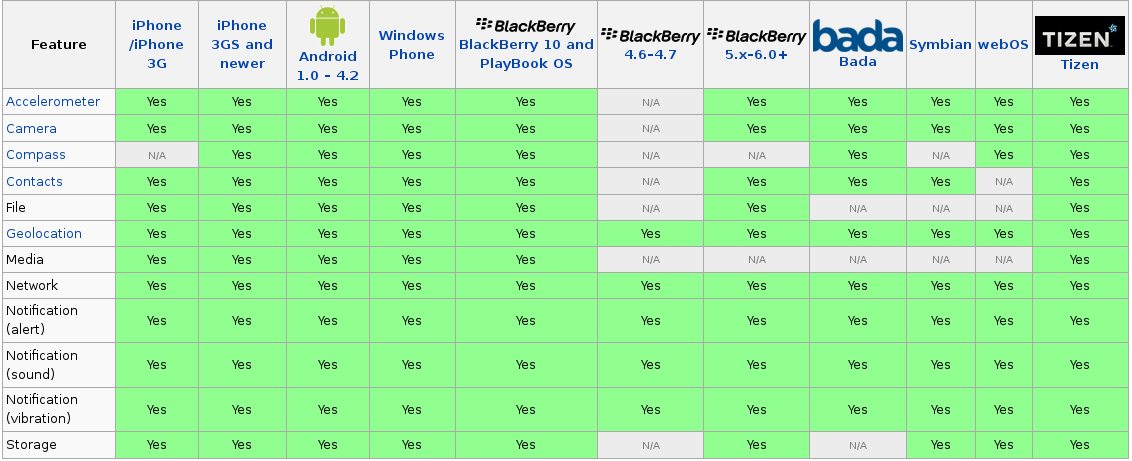
\includegraphics[width=\textwidth]{asset/img/cordovaFeatures.jpg}
               \caption{Funcionalidades implementadas para o projeto Apache Cordova.\label{fig:Cordova}}
    \end{center}
\end{figure}
%remover essa referência (sem ano e página)
Segundo JÚNIOR  utilizando as linguagens de desenvolvimento Web HTML, CSS e Javascript. Ele fornece um conjunto de API's para acesso a funções nativas do Sistema Operacional e do hardware do dispositivo, utilizando Javascript. A proposta do PhoneGap é essencial para unir as especificidades de Web com detalhes de sistemas operacionais tanto de hardware como de software.

\subsection{AMBIENTES PARA DESENVOLVIMENTO HTML5}

Após esta revisão das ferramentas  e tecnologias disponíveis, fica claro que a utilização de cada uma delas para a criação de um jogo não é um processo trivial, foi pensando nisso que algumas empresas lançaram frameworks "full stack"  (ou framework de pilha completa) para a utilização destes tipos de recursos em mobile, interoperáveis. JEFFRIES (2013) define frameworks full stack relacionados ao desenvolvimento front-end como: frameworks que nos auxiliam no completo desenvolvimento de uma aplicação, desde a interface com o usuário aos dados armazenados.
\\
Na pesquisa efetuada sobre estes frameworks full stack foram identificadas as seguientes tecnologias:

\begin{itemize}

    \item segundo (PRADO, 2012) o GWT é um framework essencialmente para o lado do cliente (cliente-side) e dá suporte à comunicação com o servidor através de RPCs Remote Procedure Calls (ou procedimento de chamadas remotas). Ele não é um framework para aplicações clássicas da web, pois deixa a implementação da aplicação web parecida com implementações em desktop. Este é utilizado em muitos produtos de grande porte como o Google Adwords e Google Wallet. Outra característica interessante é que a plataforma opera sobre a licença Apache versão 2;
    \item construct 2 -  é um editor na nuvem focado para usuários sem conhecimento prévio em programação orientado a comportamento;
    \item PlayCanvas - é uma plataformas para a construção de jogos 3D na nuvem, desenvolvida com foco em performance. Permite a hospedagem, controle de versão e publicação dos aplicativos nela criados, possibilita também a importação de modelos 3D de softwares populares como: Maya, 3ds Max e Blender;
    \item o ambiente HTML5 Development Environment (ambiente de desenvolvimento HTML5) da Intel, este fornece uma solução na nuvem, completa para o desenvolvimento em plataforma cruzada, com serviços de empacotamento, serviços para a criação e testes de aplicativos com montagem de interfaces drag and drop (Intex XDK) e biliotecas para a construção de jogos utilizando aceleração de hardware, o que garante até duas vezes mais performance que aplicativos mobile baseados em Web tradicionais. Esta solução é free, open source e funciona  através de um plugin para o Google Chrome, ou seja, o desenvolvimento também é multiplataforma e devido ao fato de os binários ficarem hospedados na nuvem, possibilitou a  Intel criar compiladores para cada uma das plataformas disponibilizadas pelo PhoneGap, que é o framework polyfill utilizado na solução.
\end{itemize}

\subsection{METODOLOGIA DE DESENVOLVIMENTO DE SOFTWARE PARA A CONSTRUÇÃO DE GAMES}

Como o jogo é um software complexo demanda-se a utilização de metodologias de engenharia de software, dentre os processos de software mais conhecidos academicamente destacamos:


\begin{itemize}
    \item OpenUP: este é bem detalhado e de característica iterativa e incremental. Gerando assim, um levantamento mais apurado dos riscos, requisitos e outros detalhes do sistema e a criação incremental do sistema, com requisitos maleáveis;
    \item Cascata: processo antigo, caracteriza-se por ser pouco maleável aos requisitos mapeados posteriormente ao processo de análise;
    \item Processo ágil - SCRUM: sua utilização é flexível e sendo um método àgil especifica pouca documentação, ou como dizem, somente a documentação necessária, este processo é bem conhecido e aceito na comunidade de desenvolvimento de software. Suas principais características são: divisão do processo de desenvolvimento através uma série de iterações chamadas sprints. Cada sprint consiste tipicamente em duas a quatro semanas. É bem aplicado a projetos que mudam constantemente e que demandam rápidas adaptações;
    \item Processo ágil – XP: tem muitas características similares ao SCRUM por este também ser um processo ágil. Dentre suas especifidades destaca-se: versões frequentes, pequenos ciclos de desenvolvimento que buscam aumentar a produtividade, indroduzem checkpoints onde os clientes podem agregar novas funcionalidades;
\end{itemize}

\subsection{USABILIDADE E TRANSPARÊNCIA}

    Conceitos de usabilidade, quando relativos ao desenvolvimento multiplataforma, devem levar em questão inúmeros fatores ou “dimensões” como:

\begin{itemize}
    \item Atores: ex – seus números, interesses, as atividades de cada um;
    \item Plataformas: ex – tipos de dispositivos, número de dispositivos, seus recursos: tamanho da tela, capacidade de som;
    \item Ambientes: ex – localização, propriedades de localização: barulho do ambiente, iluminação;
    \item Recursos do sistema: ex – disponibilidade de acesso à internet, latência de banda, CPU, memória.

\end{itemize}


Estes contextos variam em todas as dimensões. Por exemplo, um PDA quando segurado em uma mão perto de um dispositivo eletrônico, pode se tornar um controle universal daquele aparelho (PATERNÒ, 2003).
\\
	O conceito predominante relativo ao desenvolvimento de aplicativos multiplataforma que leva em consideração a usabilidade é a técnica de desenvolvimento model-based (baseado em modelos), consiste em fornecer suporte a recursos dinâmicos para uma aplicação. Segundo (BERTI, 2003), arquiteturas model-based, podem representar uma solução eficaz para problemas de usabilidade multi-plataforma. Vários sistemas de construção de interfaces a implementam, todavia esta também pode ser utilizada como conceito arquitetural para os mais variados projetos de software. Alguns produtos que utilizam construção baseada em modelos são: Fuse, Humanoid, Mastermind, Mobi-D, Tadeus, Dellach, Teresa e Trident (LUYTEN, 2004).
\\
	Em suma a arquitetura é baseada em múltiplos níveis de abstração onde cabe aos desenvolvedores detalharem os requisitos de entrada e saída dos dispositivos, os usuários a definirem suas preferências e então o sistema deve escolher a forma de iteração mais apropriada levanto em consideração os fatores anteriores.
\\
	O HTML5, não provê técnicas para o desenvolvimento baseado em modelos, nativamente, ficando a par do desenvolvedor desenvolver este recurso se assim desejar.


\subsection{TRABALHOS SIMILARES}

O browserquest da Mozilla é um jogo de RPG 8-bits focado em demonstrar na prática a utilização de muitos recursos do HTML5, este trabalho se assemelha razoavelmente ao browserquest; todavia, o browserquest não tem versão estável para a maioria dos dispositivos mobile e também distingue-se por não guardar algumas informações relativas ao estado como o posicionamento, impossibilitando assim, a experiência transparente proposta neste trabalho.
\\
	JSWars é um jogo clássico de tiro, escrito especialmente para demonstrar 	o poder do HMLT5 nos navegadores modernos (WAGNER, 2013). O trabalho aborda conceitos interessantes como física, áudio, vídeo e entrada de comandos por teclado, todavia o aplicativo não é interoperável entre dispositivos, nem fornece a perspectiva de continuidade que este trabalho propõe. Para a construção o autor utilizou javascript puro, sem auxílio de nenhuma biblioteca adicional.
\\
	Angry Birds é um título de bastante renome, este jogo foi originalmente desenvolvido para IOS, todavia, este foi portado para HTML5. O jogo faz bastante utilização de física, e como motor gráfico, utiliza o WebGL em 2D. Assim como o trabalho anterior, este não aborda o conceito de continuidade de dispositivos, havendo simplesmente uma versão para navegadores, sem utilizar recursos específicos de plataforma (HAWKES, 2013).
\\
	(SILVA,2010), demostra a utilização de HTML5 para a criação de jogos simples, todavia seu trabalho não se foca nas diferenças entre uma plataforma e outra.

\section{METODOLOGIA}
%como vou  atingir os objetivos

Primeiramente há de ser feita uma pesquisa de caráter explanatório, relativo a técnicas, ferramentas e conceitos importantes, na construção de jogos e usabilidade multiplataforma. Este tipo de pesquisa foi selecionado pois proporciona uma aproximação do pesquisador com o tema, visando melhor familiaridade com o fenômeno ou assunto (LEMÕNS et all., 2012). Neste passo pretende-se englobar o estudo das tecnologias mencionadas nos objetivos específicos: canvas, àudio, vídeo e controle de entrada, física, frameworks de desenvolvimento de jogos em HTML5, bibliotecas de detecção de recursos, tecnologias para preenchimento de gaps HTML. Também através de revisão bibliográfica, pretende-se identificar as melhores formas de explorar a interação do usuário nos diferentes dispositivos e plataformas.
\\
	O segundo passo reside na análise e construção do software em si, levando em consideração os estudos anteriormente efetuados. Haverá de se fazer uma análise e seleção das melhores ferramentas OpenSource disponíveis.
\\
	Através de um processo de software, há de se efetuar a análise e geração de artefatos que melhor mapeiem os requisitos e aspectos do jogo. Depois do período de análise, iniciar-se-á o processo de desenvolvimento, este consistirá em duas etapas subdivididas em iterações. Primeiramente há de se fazer a elaboração de um protótipo utilizando de imagens e audio de características livre na internet; após o protótipo criado, pretende-se então construir os modelos reais, bem como desenvolver a versão final, utilizando como base o protótipo. Com o software desenvolvido, far-se-à a exportação dos binários para as plataformas que suportem aplicativos nativos em HTML5 e disponibilização da aplicação online.
\\
	Ao final do desenvolvimento será feito um levantamento textual à respeito dos problemas e acertos da implementação do HTML5 encontrados durante as etapas de construção e pesquisa do projeto. Também há de ser desenvolvido um texto descritivo abordando as diferenças de implementação do controle de movimento e da interface de usuário afim de demonstrar como estes requisitos foram atendidos e quais as customizações necessárias para atendê-los nas diferentes plataformas.
\\
	Por fim, há de ser criada  uma tabela comparativa a qual exponha as funcionalidades com características dependentes de plataforma e informe se o atendimento da funcionalidade obteve êxito e como se chegou a este resultado, bem como quais outras soluções seriam possíveis. Tendo como fundamento este artefato, se fará uma análise qualitativa dos trunfos e limitações deste tipo de arquitetura para o desenvolvimento de jogos transparentes de plataforma, que oferecem experiências contínuas.

\section{CRONOGRAMA}

O cronograma foi especificado de acordo com o detalhado na metodologia, suas datas estão especificadas de acordo com dias úteis disponíveis no calendário.


\begin{table}[!htbp]
                           \begin{center}
                \begin{tabular}{ | l | l | l | l | l |}
                \hline
                \textbf{Identificador}& \textbf{Tarefa} &  \textbf{Duração} & \textbf{Início} & \textbf{Término} \\  \hline
                1 & Concepção & 5 dias & 1 agosto & 7 agosto \\  \hline
                2 & Elaboração & 15 dias & 8 agosto & 29 agosto \\  \hline
                3 & Contrução & 15 dias & 30 agosto & 19 setembro \\  \hline
                4 & Contrução & 10 dias & 31 agosto & 3 outubro \\ \hline
                  & Total & 45 dias & 1 agosto & 3 outubro \\
                \hline
                \end{tabular}
            \end{center}
               \caption{Cronograma do projeto. \label{fig:Cordova}}
\end{table}

\newpage


%colocar em ordem alfabética de autores
%separar autores por ; e sobrenome/nome por virgula
% mais de 3 autores: SOBRENOME, Nome et al.
% CITAÇÕES DIRETAS
%citações no padrão: "Texto citado" (GARCIA, 2006, p.380)
%para mais de 3 linhas de citação deve-se utilizar 4cm de margem
%esquerda em tamanho 10
% CITAÇÕES INDIRETAS
%
% Para Oliveira e Oliveira (2006, p.19), a finalidade de blablabla
%
bibliotecam\begin{thebibliography}{99}

\bibitem{AK}
AK, Sheela
\emph{ Global Gaming Market Is Expected to Reach USD 117.9 Billion by 2015: Transparency Market Research}.
Disponível em: http://www.prnewswire.com/news-releases/global-gaming-market-is-expected-to-reach-usd-1179-billion-by-2015-transparency-market-research-169284526.html
Acesso em: Jul 2012.

 
\bibitem{BUCHMAN}
BUCHMAN, Debra D; FUNK, Jeanne B. 
\emph{VIDEO AND COMPUTER GAMES IN THE "90S: CHILDREN'S TIME COMMITMENT & GAME PREFERENCE}. 
Health and Human Services Department (HHS), 2013.


\bibitem{KURYANOVICH}
  KURYANOVICH, Egor; SHALOM Shy, et all.
  \emph{The State of Open Web Games}.
  Addison Wesley, Massachusetts, pg. 12,
  ISBN: 978-1-4302-3978-9,
  2012.

\bibitem{SILVA}
SILVA, Jucimar Maria Júnior; FIRMINO, Emiliano Carlos M.
  \emph{Desenvolvimento de jogos em HTML5}.
  Coordenação da engenharia da Computação,
  Univerisdade Federal do Amazonas,
  Amazonas,
  2010.

  \bibitem{SHANKAR}
SHANKAR, Aditya Ravi .
  \emph{Pro HTML5 Games}.
 ISBN: 978-1-4302-4710-4, p. 39-64,
 2012.

 \bibitem{TABUSCA}
TABUSCA, Alexandru
  \emph{THE NEW “UNIVERSAL TRUTH” OF THE WORLD WIDE WEB}.
American University, School of Computer Science for
Business Management, Bucharest, 2013

 \bibitem{PRALL}
PRALL, Chandler
  \emph{JavaScript Physics Engines Comparison}.
Disponível em: http://www.htmlgoodies.com/html5/client/javascript-physics-engines-comparison.html#fbid=AAlTVDXjb40
Acesso em: Jul 2013.

 \bibitem{VGChartz}
VGChartz
  \emph{Global sales (in millions of units) per game}.
Disponível em: http://www.vgchartz.com/gamedb/
Acesso em: Jul 2012.



\bibitem{SILVA2011} 
SILVA, Maurício Samy
\emph{HTML5 A linguagemEM DE MARCAÇÃO QUE REVOLUCIONOU A WEB}. 
Editora novatec, p. 15, 2011.

\bibitem{FRANZINI} 
 FRANZINI, Fernando 
 \emph{Nova tendência de aplicativos móveis web}.  Disponível em:
[http://www.infobase.com.br/nova-tendencia-de-aplicativos-moveis-web/]. Acesso em: jun,
2013.

\bibitem{JEFFRIES}
JEFFRIES, Ron 
\emph{Full-Stack frameworks vs. Non Full-Stack frameworks}.
Disponível em [http://codingarchitect.wordpress.com/2012/10/22/full-stack-frameworks-vs-non-full-stack-frameworks/], Acesso em: jun, 2013.


\bibitem{JÚNIOR} 
JÚNIOR, Gesmar de Paula Santos; OLIVEIRA, Luciene Chagas; CARDOSO, Alexandre; LAMOUNIER, Edgard Afonso.
\emph{Aplicação Multiplataforma da Realidade Aumentada Móvel para Geolocalização utilizando o PhoneGap}.
Programa de Pós Gradução em Engenharia Elétrica
Universidade Federal de Uberlândia, rograma de Pós Gradução em Engenharia Elétrica
Universidade Federal de Uberlândia, Uberlândia, Minas Gerais.



\bibitem{PRADO}
PRADO, Ely Fernando
\emph{Introdução ao Desenvolvimento de Games com GWT e HTML5}. 
Departamento de Computação, Universidade Federal de São Carlos (UFSCar) São Carlos, SP, 2012.


\bibitem{RENYO}
RENYO Emanuel Montero 
\emph{MODEL-DRIVEN GAME DEVELOPMENT: 2D PLATFORM GAME PROTOTYPING}. 
Departamento de Sistemas Informáticos y Computación. Universidad Politécnica de Valencia,Valencia, España, 2006.



\bibitem{HERMIDA}
HERMIDA, Alfred 
Japan leads mobile game craze. BBC News, 2003. Acesso em: jun 2013.

\bibitem{EvolutionOnGames}
\emph{A incrível evolução de videogames de console}. 
Disponível em: [http://www.failwars.blog.br/nerd-feelings/incrvel-evoluo-dos-vdeo-games-de-console-de-1967-2012/] Acesso em: jun, 2013.

 \bibitem{WEINTRAUB}
WEINTRAUB, Seth
  \emph{Industry first: Smartphones pass PCs in sales}.
Disponível em: http://tech.fortune.cnn.com/2011/02/07/idc-smartphone-shipment-numbers-passed-pc-in-q4-2010/
Acesso em: Jul 2012.

\bibitem{ZICO}
ZICO, Mário Lucio 
\emph{A História dos Jogo}. 
Disponível em [http://www.jogos.antigos.nom.br/artigos.asp], Acesso em: jun 2013.



\end{thebibliography}

\printindex[not]
\printindex[aut][Here is a prologue for the author index.
Note that it is set in a single column at the top of the
first page of the index.]

\printindex[list]

\printindex
\end{document}





